\documentclass[11pt, a4paper]{article}

\usepackage{amsmath, amssymb, titling}
\usepackage[margin=2.5cm]{geometry}
\usepackage[colorlinks=true, linkcolor=black, urlcolor=black, citecolor=black]{hyperref}
\usepackage{url}
\usepackage{graphicx}
\usepackage{caption}
\usepackage{subcaption}
\usepackage{float}
\usepackage{cancel}
\usepackage{fancyhdr, lastpage}
\usepackage{fourier-orns}
\usepackage{xcolor}
\usepackage{nomencl}
\makenomenclature
\usepackage{etoolbox}
\usepackage{sidecap}
\usepackage{adjustbox}
\usepackage{listings}
\usepackage{matlab-prettifier}
\usepackage[T1]{fontenc}

\sidecaptionvpos{figure}{c}
\setlength{\headheight}{18.2pt}
\setlength{\nomlabelwidth}{1.5cm}

\renewcommand\maketitlehooka{\null\mbox{}\vfill}
\renewcommand\maketitlehookd{\vfill\null}

\renewcommand{\headrule}{\vspace{-5pt}\hrulefill\raisebox{-2.1pt}{\quad\leafleft\decoone\leafright\quad}\hrulefill}
\newcommand{\parder}[2]{\frac{\partial {#1}}{\partial {#2}}}
% \renewcommand\nomgroup[1]{%
%   \item[\bfseries
%   \ifstrequal{#1}{F}{Far--Away Properties}{%
%   \ifstrequal{#1}{N}{Dimensionless Numbers}{%
%   \ifstrequal{#1}{M}{Matrices}{%
%   \ifstrequal{#1}{D}{Diagonals}{%
%   \ifstrequal{#1}{V}{Vectors}{%
%   \ifstrequal{#1}{P}{Dimensionless Average Properties}{}}}}}}
% ]}

\title{Intro to Turbulent Flow \\ HW2}
\author{Almog Dobrescu ID 214254252}

% \pagestyle{fancy}
\cfoot{Page \thepage\ of \pageref{LastPage}}

\begin{document}

\thispagestyle{empty}
\maketitle
\newpage

\pagenumbering{roman}
% \setcounter{page}{1}

\tableofcontents
\vfil
\listoffigures
\vfil
\lstlistoflistings
\newpage

\printnomenclature
\newpage

\pagestyle{fancy}
\pagenumbering{arabic}
\setcounter{page}{1}

\section{Stationarity and Ergodicity}
For a random process to be stationary, it needs to fulfill the following conditions:
\begin{enumerate}
    \item $\displaystyle\mathbb{E}{\left\{{x_k}_{\left(t\right)}\right\}}=\text{constant}$
    \item $\displaystyle Q_{\left(t,t+s\right)}=\mathbb{E}\left\{{x_k}_{\left(t\right)}{x_k}_{\left(t+s\right)}\right\}=Q_{\left(s\right)}$
\end{enumerate}
To determine if a random process is ergodic the following condition needs to be met:
\begin{enumerate}
    \item $\displaystyle\lim_{T\rightarrow\infty}\frac{1}{T}\int_{0}^{T}{Q_{\left(\hat{s}\right)}d\hat{s}}=0$
\end{enumerate}
\subsection{Random Process \#1}
\begin{equation}
    x_k=a_k\sin{\left(2\pi ft+\theta\right)}
\end{equation}
Where:
\begin{equation}
    a_k\sim U\left[0,1\right]
\end{equation}
\subsubsection{Statinarity}
The expectation operator for $x_k$ is given by:
\begin{equation}
    \begin{array}{rcl}
        \displaystyle \mathbb{E}{\left\{{x_k}_{\left(t\right)}\right\}} & = & \displaystyle \int_{0}^{1}{a\sin{\left(2\pi ft+\theta\right)}da} \\\\
        & = & \displaystyle \left[\frac{1}{2}a^2\sin{\left(2\pi ft+\theta\right)}\right]_0^1 \\\\
        & = & \displaystyle \frac{1}{2}\sin{\left(2\pi tf+\theta\right)}\ne\text{const}
    \end{array}
\end{equation}
\begin{equation*}
    \begin{array}{c}
        \Downarrow \\
        \boxed{$\text{Not stationary}$}
    \end{array}
\end{equation*}
\subsubsection{Ergodicity}
The covariance function is given by:
\begin{equation}
    \begin{array}{rcl}
        Q_{\left(t,t+s\right)} & = & \displaystyle \mathbb{E}\left\{{x_k}_{\left(t\right)}{x_k}_{\left(t+s\right)}\right\} \\\\
        & = & \displaystyle \mathbb{E}\left\{a_k\sin{\left(2\pi ft+\theta\right)}a_k\sin{\left(2\pi f\left(t+s\right)+\theta\right)}\right\} \\\\
        & \Downarrow & \displaystyle \sin{\left(\alpha\right)}\sin{\left(\beta\right)}=\frac{1}{2}\left[\cos\left(\alpha-\beta\right)+\cos\left(\alpha+\beta\right)\right] \\\\
        & = & \displaystyle \mathbb{E}\left\{a_k^2\frac{1}{2}\left[\cos\left(2\pi ft+\theta-2\pi f\left(t+s\right)-\theta\right)-\cos\left(2\pi ft+\theta+2\pi f\left(t+s\right)+\theta\right)\right]\right\} \\\\
        & = & \displaystyle \int_{0}^{1}{a^2\frac{1}{2}\left[\cos\left(2\pi fs\right)-\cos\left(4\pi ft+2\pi fs+2\theta\right)\right]da} \\\\
        & = & \displaystyle \int_{0}^{1}{a^3\frac{1}{6}\left[\cos\left(2\pi fs\right)-\cos\left(4\pi ft+2\pi fs+2\theta\right)\right]da}\ne Q_{\left(s\right)}
    \end{array}
\end{equation}
\begin{equation*}
    \begin{array}{c}
        \Downarrow \\
        \boxed{$\text{Not ergodic}$}
    \end{array}
\end{equation*}
\subsection{Random Process \#2}
\begin{equation}
    x_k=a\sin{\left(2\pi ft+\theta_k\right)}
\end{equation}
Where:
\begin{equation}
    \theta_k\sim U\left[0,2\pi\right]
\end{equation}
\subsubsection{Statinarity}
The expectation operator for $x_k$ is given by:
\begin{equation}
    \begin{array}{rcl}
        \displaystyle \mathbb{E}{\left\{{x_k}_{\left(t\right)}\right\}} & = & \displaystyle \int_{0}^{2\pi}{\frac{1}{2\pi}\alpha\sin{\left(2\pi ft+\theta\right)}d\theta} \\\\
        & = & \displaystyle \left[-\frac{1}{2\pi}\alpha\cos{\left(2\pi ft+\theta\right)}\right]_0^{2\pi} \\\\
        & = & \displaystyle -\frac{1}{2\pi}\alpha\cos{\left(2\pi ft+2\pi\right)}+\frac{1}{2\pi}\alpha\cos{\left(2\pi ft+0\right)} \\\\
        & = & 0=\text{const}
    \end{array}
\end{equation}
The covariance function is given by:
\begin{equation}
    \begin{array}{rcl}
        Q_{\left(t,t+s\right)} & = & \displaystyle \mathbb{E}\left\{{x_k}_{\left(t\right)}{x_k}_{\left(t+s\right)}\right\} \\\\
        Q_{\left(t,t+s\right)} & = & \displaystyle \mathbb{E}\left\{a\sin{\left(2\pi ft+\theta_k\right)}a\sin{\left(2\pi f\left(t+s\right)+\theta_k\right)}\right\} \\\\
        & \Downarrow & \displaystyle \sin{\left(\alpha\right)}\sin{\left(\beta\right)}=\frac{1}{2}\left[\cos\left(\alpha-\beta\right)+\cos\left(\alpha+\beta\right)\right] \\\\
        & = & \displaystyle \mathbb{E}\left\{a^2\frac{1}{2}\left[\cos\left(2\pi ft+\theta_k-2\pi f\left(t+s\right)-\theta_k\right)-\cos\left(2\pi ft+\theta_k+2\pi f\left(t+s\right)+\theta_k\right)\right]\right\} \\\\
        & = & \displaystyle \int_{0}^{2\pi}{a^2\frac{1}{4\pi}\left[\cos\left(2\pi ft+\theta-2\pi f\left(t+s\right)-\theta\right)-\cos\left(2\pi ft+\theta+2\pi f\left(t+s\right)+\theta\right)\right]d\theta} \\\\
        & = & \displaystyle \int_{0}^{2\pi}{\left[a^2\frac{1}{4\pi}\cos\left(2\pi fs\right)-a^2\frac{1}{4\pi}\cos\left(4\pi ft+2\theta+2\pi fs\right)\right]d\theta} \\\\
        & = & \displaystyle \left[a^2\frac{1}{4\pi}\cos\left(2\pi fs\right)\theta-a^2\frac{1}{8\pi}\sin\left(4\pi ft+2\theta+2\pi fs\right)\right]_0^{2\pi} \\\\
        & = & \displaystyle a^2\frac{1}{2}\cos\left(2\pi fs\right)-a^2\frac{1}{8\pi}\sin\left(4\pi ft+4\pi+2\pi fs\right)+a^2\frac{1}{8\pi}\sin\left(4\pi ft+2\pi fs\right) \\\\
        & = & \displaystyle \frac{a^2}{2}\cos\left(2\pi fs\right)=Q_{\left(s\right)}\qquad\blacksquare
    \end{array}
\end{equation}
\begin{equation*}
    \begin{array}{c}
        \Downarrow \\
        \boxed{$\text{Stationary}$}
    \end{array}
\end{equation*}
\subsubsection{Ergodicity}
To prove an ergodic process we need to check the next limit:
\begin{equation}
    \begin{array}{rcl}
        \displaystyle \lim_{T\rightarrow\infty}\frac{1}{T}\int_{0}^{T}{Q_{\left(\hat{s}\right)}d\hat{s}} & = & \displaystyle \lim_{T\rightarrow\infty}\frac{1}{T}\int_{0}^{T}{\frac{a^2}{2}\cos\left(2\pi f\hat{s}\right)d\hat{s}} \\\\
        & = & \displaystyle \lim_{T\rightarrow\infty}\frac{1}{T}\left[\frac{a^2}{4\pi f}\sin\left(2\pi f\hat{s}\right)\right]_0^T \\\\
        & = & \displaystyle \lim_{T\rightarrow\infty}\frac{1}{T}\frac{a^2}{4\pi f}\sin\left(2\pi fT\right)=0\qquad\blacksquare
    \end{array}
\end{equation}
\begin{equation*}
    \begin{array}{c}
        \Downarrow \\
        \boxed{$\text{Ergodic}$}
    \end{array}
\end{equation*}
\subsection{Random Process \#3}
\begin{equation}
    x_k=a_k\sin{\left(2\pi ft+\theta_k\right)}
\end{equation}
Where:
\begin{equation}
    \begin{matrix}
        a_k\sim U\left[0,1\right] && \theta_k\sim U\left[0,2\pi\right]
    \end{matrix}
\end{equation}
\subsubsection{Statinarity}
The expectation operator for $x_k$ is given by:
\begin{equation}
    \begin{array}{rcl}
        \displaystyle \mathbb{E}{\left\{{x_k}_{\left(t\right)}\right\}} & = & \displaystyle \int_{0}^{2\pi}{\frac{1}{2\pi}\int_{0}^{1}{a\sin{\left(2\pi ft+\theta\right)}da}d\theta} \\\\
        & = & \displaystyle \int_{0}^{2\pi}{\frac{1}{2\pi}\left[\frac{a^2}{2}\sin{\left(2\pi ft+\theta\right)}\right]_0^1d\theta} \\\\
        & = & \displaystyle \int_{0}^{2\pi}{\frac{1}{4\pi}\sin{\left(2\pi ft+\theta\right)}d\theta} \\\\
        & = & \displaystyle \left[-\frac{1}{4\pi}\cos{\left(2\pi ft+\theta\right)}\right]_0^{2\pi}=0=\text{const}
    \end{array}
\end{equation}
The covariance function is given by:
\begin{equation}
    \begin{array}{rcl}
        Q_{\left(t,t+s\right)} & = & \displaystyle \mathbb{E}\left\{{x_k}_{\left(t\right)}{x_k}_{\left(t+s\right)}\right\} \\\\
        Q_{\left(t,t+s\right)} & = & \displaystyle \mathbb{E}\left\{a_k\sin{\left(2\pi ft+\theta_k\right)}a_k\sin{\left(2\pi f\left(t+s\right)+\theta_k\right)}\right\} \\\\
        & \Downarrow & \displaystyle \sin{\left(\alpha\right)}\sin{\left(\beta\right)}=\frac{1}{2}\left[\cos\left(\alpha-\beta\right)+\cos\left(\alpha+\beta\right)\right] \\\\
        & = & \displaystyle \mathbb{E}\left\{a_k^2\frac{1}{2}\left[\cos\left(2\pi ft+\theta_k-2\pi f\left(t+s\right)-\theta_k\right)-\cos\left(2\pi ft+\theta_k+2\pi f\left(t+s\right)+\theta_k\right)\right]\right\} \\\\
        & = & \displaystyle \mathbb{E}\left\{a_k^2\frac{1}{2}\left[\cos\left(2\pi fs\right)-\cos\left(4\pi ft+2\theta_k+2\pi fs\right)\right]\right\} \\\\
        & = & \displaystyle \int_{0}^{2\pi}{\frac{1}{2\pi}\int_{0}^{1}{a^2\frac{1}{2}\left[\cos\left(2\pi fs\right)-\cos\left(4\pi ft+2\theta+2\pi fs\right)\right]da}d\theta} \\\\
        & = & \displaystyle \int_{0}^{2\pi}{\frac{1}{2\pi}\left[a^3\frac{1}{6}\left[\cos\left(2\pi fs\right)-\cos\left(4\pi ft+2\theta+2\pi fs\right)\right]\right]_0^1d\theta} \\\\
        & = & \displaystyle \int_{0}^{2\pi}{\left[\frac{1}{12\pi}\cos\left(2\pi fs\right)-\frac{1}{12\pi}\cos\left(4\pi ft+2\theta+2\pi fs\right)\right]d\theta} \\\\
        & = & \displaystyle \left[\frac{1}{12\pi}\cos\left(2\pi fs\right)\theta-\frac{1}{24\pi}\sin\left(4\pi ft+2\theta+2\pi fs\right)\right]_0^{2\pi} \\\\
        & = & \displaystyle \frac{1}{6}\cos\left(2\pi fs\right)=Q_{\left(s\right)}\qquad\blacksquare
    \end{array}
\end{equation}
\begin{equation*}
    \begin{array}{c}
        \Downarrow \\
        \boxed{$\text{Stationary}$}
    \end{array}
\end{equation*}
\subsubsection{Ergodicity}
To prove an ergodic process we need to check the next limit:
\begin{equation}
    \begin{array}{rcl}
        \displaystyle \lim_{T\rightarrow\infty}\frac{1}{T}\int_{0}^{T}{Q_{\left(\hat{s}\right)}d\hat{s}} & = & \displaystyle \lim_{T\rightarrow\infty}\frac{1}{T}\int_{0}^{T}{\frac{1}{6}\cos\left(2\pi f\hat{s}\right)d\hat{s}} \\\\
        & = & \displaystyle \lim_{T\rightarrow\infty}\frac{1}{T}\left[\frac{1}{12\pi f}\sin\left(2\pi f\hat{s}\right)\right]_0^T \\\\
        & = & \displaystyle \lim_{T\rightarrow\infty}\frac{1}{T}\frac{1}{12\pi f}\sin\left(2\pi fT\right)=0\qquad\blacksquare
    \end{array}
\end{equation}
\begin{equation*}
    \begin{array}{c}
        \Downarrow \\
        \boxed{$\text{Ergodic}$}
    \end{array}
\end{equation*}

\newpage
\section{Getting Closure}
Considering the differencing equation:
\begin{equation}
    u_{n+1}=ru_n\left(1-u_n\right)
\end{equation}
\subsection{Ensemble Average $\langle u\rangle$}
In order to calculate the ensemble average $\langle u\rangle$ we will assume that the limit $\lim_{n\rightarrow\infty}{u_n}$ exists. This means there is \emph{n} at which $u_{n+1}=u_n=u$. Hence:
\begin{equation}
    \begin{array}{rcl}
        \langle u\rangle & = & \langle u_{n+1}\rangle=\langle ru-ru^2\rangle= r\langle u\rangle-r\langle u^2\rangle \\\\
        \left(1-r\right)\langle u\rangle& = & -r\langle u^2\rangle \\\\
        \langle u\rangle& = & \displaystyle\frac{-r}{1-r}\langle u^2\rangle\qquad\blacksquare
    \end{array}
\end{equation}
Where:
\begin{itemize}
    \item $\langle u\rangle$ is the first moment
    \item $\langle u^2\rangle$ is the second moment
\end{itemize}
\subsection{Reynolds Stress}
The Reynolds stresses can be represented as the second moment and form the first subsection, it can be written as:
\begin{equation}
    \langle u\cdot u\rangle=\langle u^2\rangle=\frac{1-r}{-r}\langle u\rangle
\end{equation}
The Reynolds stress depends on the ensemble average and the variable \emph{r}.
\subsection{Solving For $\langle u\rangle$}
The first moment depends on the second moment so we can't solve it directly. Let's try to solve for the second moment:
\begin{equation}
    \begin{array}{rcl}
        \langle u\cdot u\rangle & = & \langle\left(ru-ru^2\right)\left(ru-ru^2\right)\rangle \\\\
        & = & \langle r^2u^2-r^2u^3-r^2u^3+r^2u^4\rangle \\\\
        & = & \langle r^2u^2\rangle-\langle 2r^2u^3\rangle+\langle r^2u^4\rangle \\\\
        & = & r^2\left(\langle u^2\rangle-\langle 2u^3\rangle+\langle u^4\rangle\right)
    \end{array}
\end{equation}
We see that the second moment depends on the third and fourth moments. We can conclude that each moment depends on a higher-order moment and this 'series' continues to infinity. Hence we can not solve for the first moment directly. \\
By assuming that u is normaly distributed, $N\left[\mu,\sigma\right]$, we get the following central moments: % lecture pg.24 table.1 + wiqipedia: https://en.wikipedia.org/wiki/Moment_(mathematics) & https://en.wikipedia.org/wiki/Covariance
\begin{table}[H]
    \center
    \begin{tabular}{c||c||c||c||c}
        $\langle u\rangle=\mu$ & $\sigma^2=\mathbb{E}\left\{\left(u-\mu\right)^2\right\}$ & $Q_{\left(u,v\right)}=\mathbb{E}\left\{\left(u-\mu_u\right)\left(v-\mu_v\right)\right\}$ & $\mu_3=\mathbb{E}\left\{\left(u-\mu\right)^3\right\}$ & $\mu_4=\mathbb{E}\left\{\left(u-\mu\right)^4\right\}$
    \end{tabular}
\end{table}
\begin{equation*}
    \Downarrow
\end{equation*}
\begin{equation}
    \begin{array}{c}
        \sigma^2=Q_{\left(u,u\right)}=\langle u^2\rangle-\langle u\rangle^2 \\\\
        \langle u^2\rangle=\langle u\rangle^2+\sigma^2 \\\\
        \langle u^2\rangle=\mu^2+\sigma^2
    \end{array}
\end{equation}
We also know that: 
\begin{equation}
    \begin{array}{rcl}
        \langle u^2\rangle & = & r^2\left(\langle u^2\rangle-\langle 2u^3\rangle+\langle u^4\rangle\right) \\\\
        \langle u^2\rangle & = & \displaystyle\frac{r^2}{1-r^2}\left(-2\langle u^3\rangle+\langle u^4\rangle\right)
        \label{eq: second moment}
    \end{array}
\end{equation}
What we have here are non central moments. For normal distribution we know that:
% \begin{equation}
%     \begin{matrix}
%         \displaystyle\langle u^3\rangle=\frac{b^{3+1}-a^{3+1}}{\left(3+1\right)\left(b-a\right)} & \displaystyle\text{and} & \displaystyle\langle u^4\rangle=\frac{b^{4+1}-a^{4+1}}{\left(4+1\right)\left(b-a\right)}
%     \end{matrix}
%     \label{eq: third and fourth moments}
% \end{equation}
% Where:
% \begin{itemize}
%     \item $a=0$
%     \item $b=1$
% \end{itemize}
% \begin{equation*}
%     \begin{matrix}
%         \displaystyle\langle u^3\rangle=\frac{1}{4} & \displaystyle\text{and} & \displaystyle\langle u^4\rangle=\frac{1}{5}
%     \end{matrix}
% \end{equation*}
% Substituting Eq.\ref{eq: third and fourth moments} into Eq.\ref{eq: second moment}:
% \begin{equation}
%     \begin{array}{c}
%         \langle u^2\rangle=\displaystyle\frac{r^2}{1-r^2}\left(-2\frac{1}{4}+\frac{1}{5}\right) \\\\
%         \text{and} \\\\
%         \langle u\rangle=\displaystyle\frac{r}{r-1}\langle u^2\rangle \\\\
%         \Downarrow \\
%         \mu=\displaystyle \frac{-r^3}{\left(r-1\right)\left(1-r^2\right)}\frac{3}{10}
%     \end{array}
% \end{equation}
\begin{equation}
    \begin{matrix}
        \langle u^3\rangle=\mu^3+3\mu\sigma^2 & \text{and} & \langle u^4\rangle=\mu^4+6\mu^2\sigma^2+3\sigma^4
    \end{matrix}
    \label{eq: third and fourth moments}
\end{equation}
Substituting Eq.\ref{eq: third and fourth moments} into Eq.\ref{eq: second moment}:
\begin{equation}
    \begin{array}{c}
        \mu^2+\sigma^2=\displaystyle\frac{r^2}{1-r^2}\left(-2\left(\mu^3+3\mu\sigma^2\right)+\mu^4+6\mu^2\sigma^2+3\sigma^4\right) \\\\
        \text{and} \\\\
        \mu=\displaystyle\frac{r}{r-1}\left(\mu^2+\sigma^2\right)
    \end{array}
\end{equation}
The ensemble average can be calculated using a numerical system of equations solver.
\subsection{Numerical Verification}
Let's compare the analytical solution to a numerical one:
\begin{figure}[H]
    \centering
    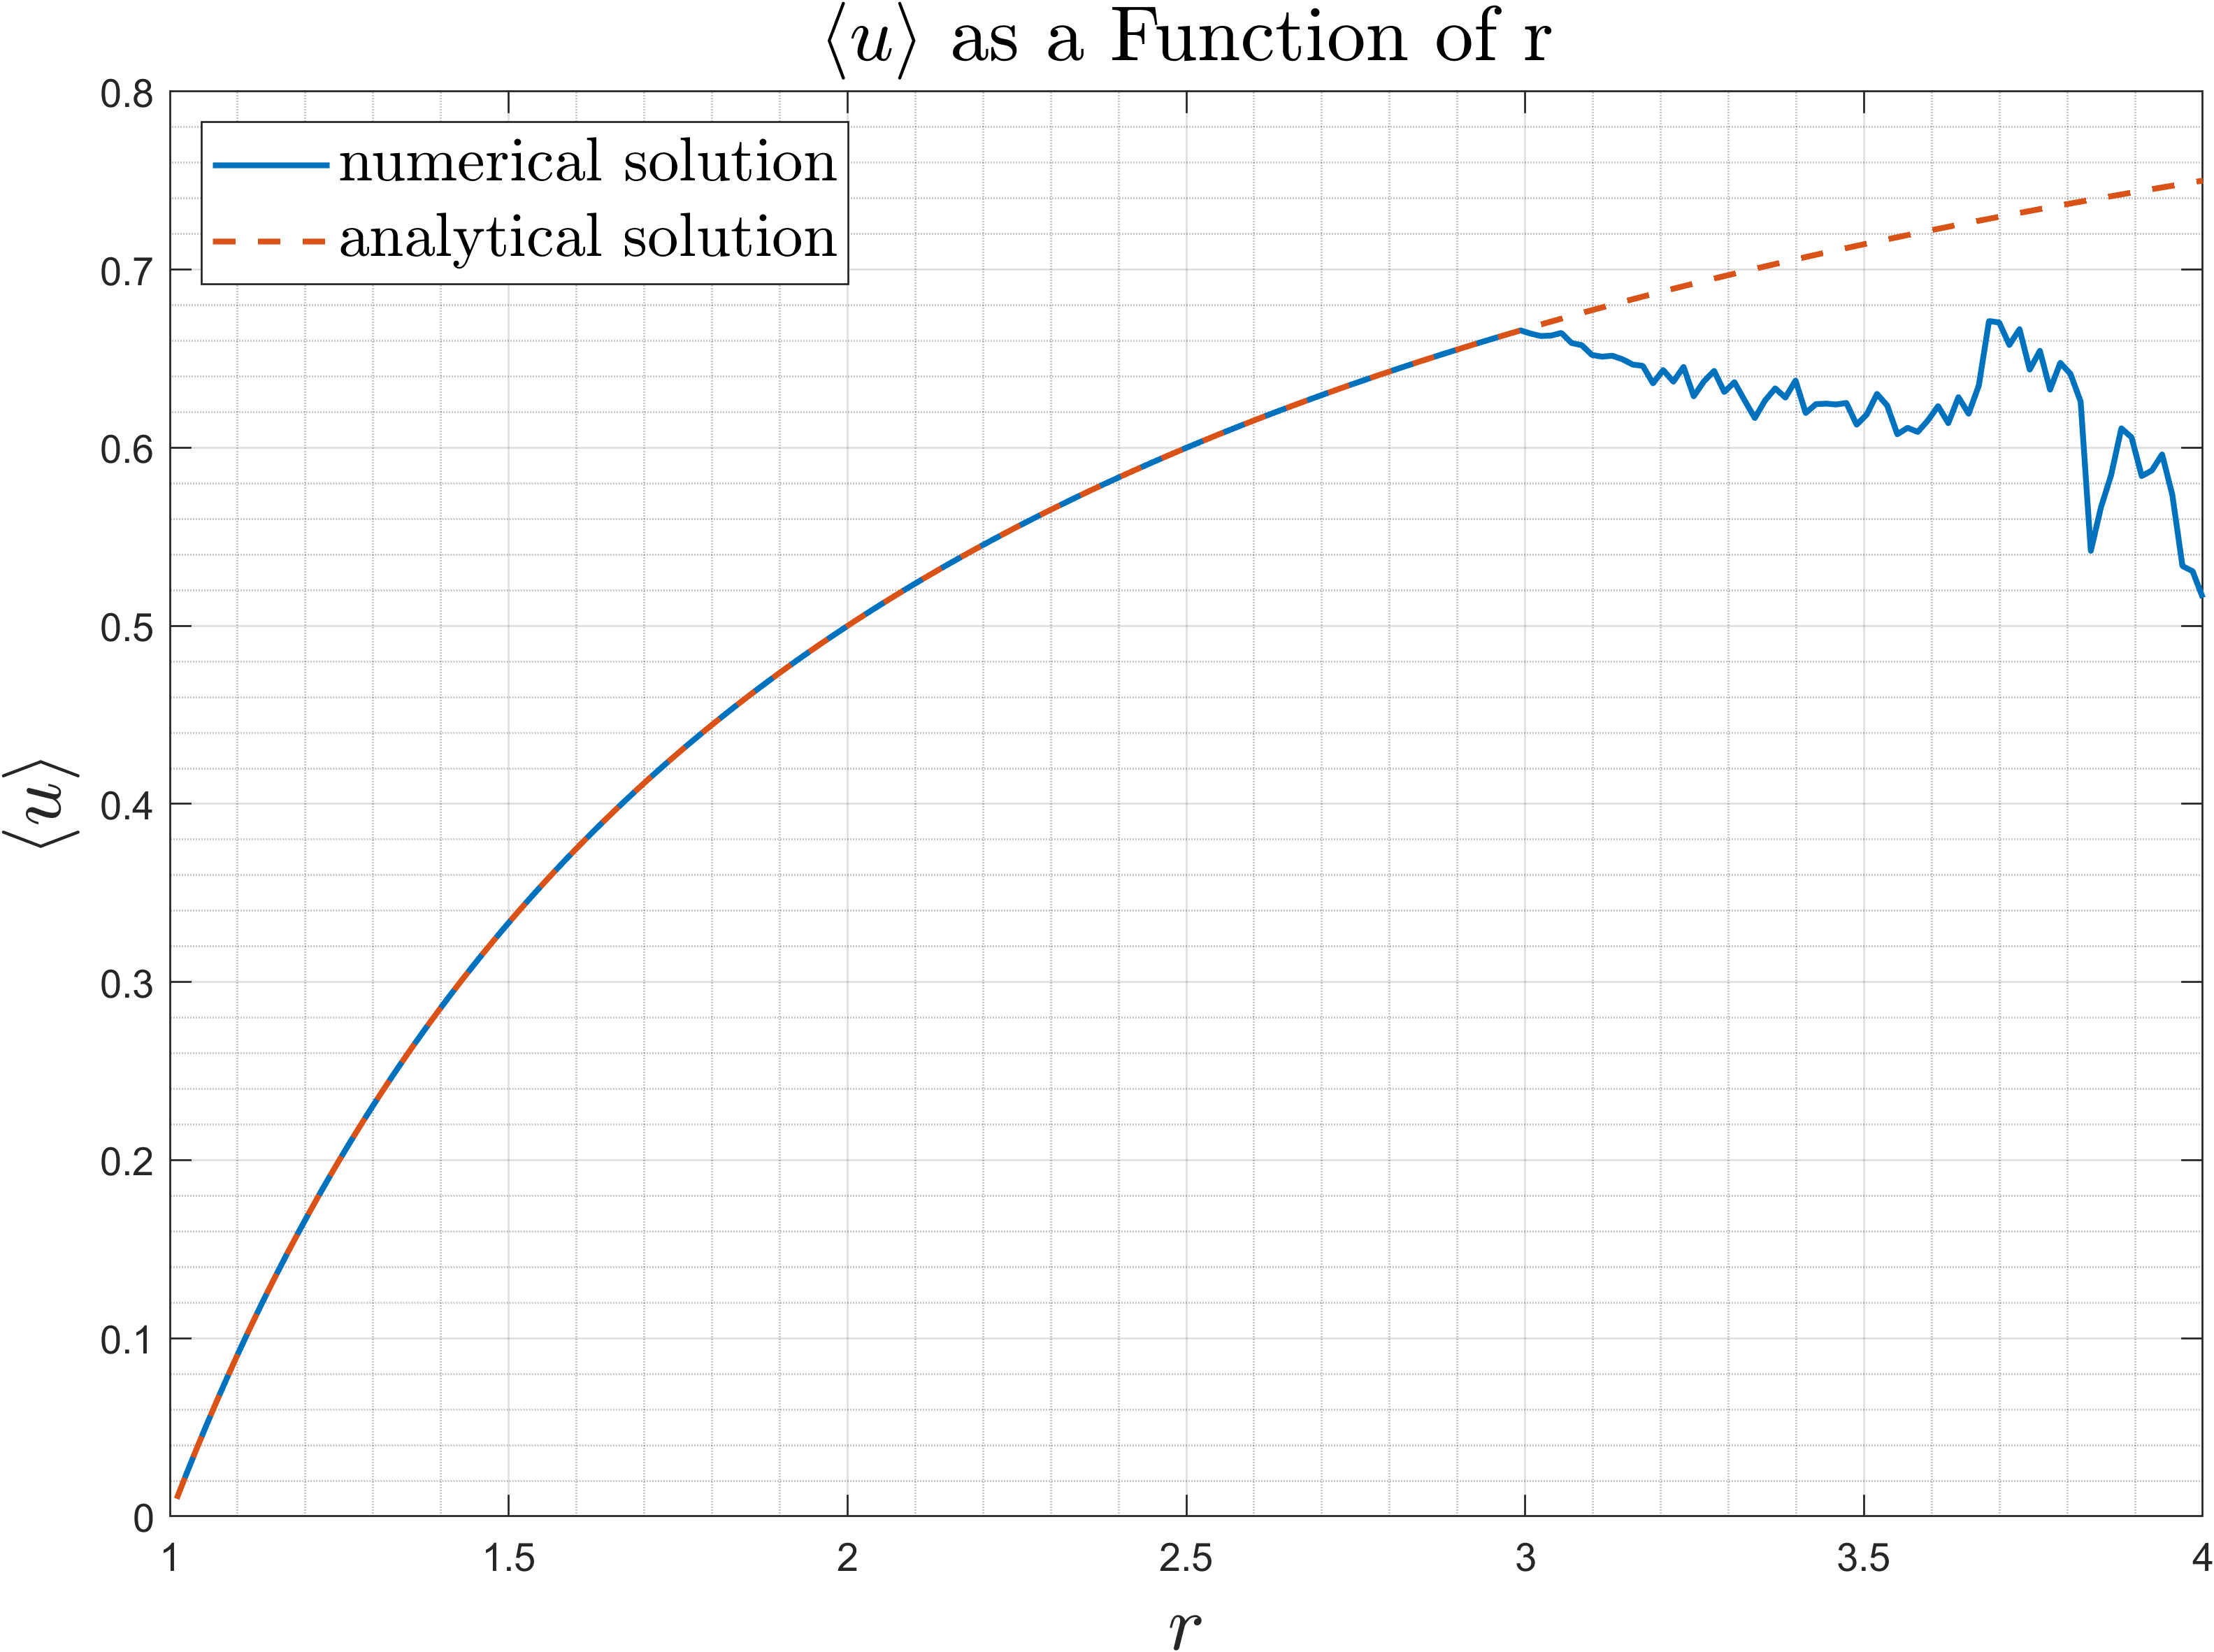
\includegraphics[width=0.7\textwidth]{images/Q2.4.png}
    \caption{Calculating PDF}
    \label{fig: calculating pdf}
\end{figure}
\noindent The figure shows that indeed the analytically calculated solution feet the numerical one for all $1<r<3$. This means that the ensemble average can be consider as normally distributed for $r<3$.

\newpage
\section{Scalar TKE Equation}
Considering the instantaneous transport equation for a passive scalar $\tilde{T}$:
\begin{equation}
    \parder{\tilde{T}}{t}+\parder{}{x_j}\left(\tilde{T}\tilde{u}_j\right)=\alpha\parder{^2\tilde{T}}{x^2_j}
\end{equation}
Where:
\begin{itemize}
    \item $\tilde{T}=\bar{T}+T$
    \item $\tilde{u}=\bar{u}+u$
    \item $\tilde{\left(\cdot\right)}$ - instantaneous
quantity
    \item $\bar{\left(\cdot\right)}$ - ensemble average
    \item $\left(\cdot\right)$ - fluctuating component representing the
turbulence
\end{itemize}
In order to describe the magnitude of the fluctuations we will derive an equivalent to the TKE for the temperature fluctuations, $\frac{1}{2}\bar{T}^2$:
\begin{equation}
    \begin{array}{rcl}
        \displaystyle \parder{\bar{T}+T}{t}+\parder{}{x_j}\left(\left(\bar{T}+T\right)\left(\bar{u}_j+u_j\right)\right) & = & \displaystyle \alpha\parder{^2}{x^2_j}\left(\bar{T}+T\right) \\\\
        \displaystyle \parder{\bar{T}}{t}+\parder{T}{t}+\parder{}{x_j}\left(\bar{T}\bar{u}_j+\bar{T}u_j+T\bar{u}_j+Tu_j\right) & = & \displaystyle \alpha\parder{^2\bar{T}}{x^2_j}+\alpha\parder{^2T}{x^2_j}
        \label{eq: given equation}
    \end{array}
\end{equation}
Let's ensemble average: % lecture pg.42 eq.18
\begin{equation}
    \begin{array}{c}
        \overline{\displaystyle \parder{\bar{T}}{t}+\parder{T}{t}+\parder{}{x_j}\left(\bar{T}\bar{u}_j+\bar{T}u_j+T\bar{u}_j+Tu_j\right)=\displaystyle \alpha\parder{^2\bar{T}}{x^2_j}+\alpha\parder{^2T}{x^2_j}} \\\\
        \overline{\displaystyle \parder{\bar{T}}{t}}+\overline{\displaystyle\parder{T}{t}}+\overline{\displaystyle\parder{}{x_j}\left(\bar{T}\bar{u}_j+\bar{T}u_j+T\bar{u}_j+Tu_j\right)}=\overline{\displaystyle \alpha\parder{^2\bar{T}}{x^2_j}}+\overline{\displaystyle\alpha\parder{^2T}{x^2_j}} \\\\
        \displaystyle \parder{\bar{T}}{t}+\displaystyle\parder{}{x_j}\left(\overline{\bar{T}\bar{u}_j+\bar{T}u_j+T\bar{u}_j+Tu_j}\right)=\displaystyle \alpha\parder{^2\bar{T}}{x^2_j} \\\\
        \displaystyle \parder{\bar{T}}{t}+\displaystyle\parder{}{x_j}\left(\bar{T}\bar{u}_j+\overline{Tu_j}\right)=\displaystyle \alpha\parder{^2\bar{T}}{x^2_j} \\\\
        \displaystyle \parder{\bar{T}}{t}+\displaystyle\parder{\bar{T}\bar{u}_j}{x_j}+\parder{\overline{Tu_j}}{x_j}=\displaystyle \alpha\parder{^2\bar{T}}{x^2_j}
        \label{eq: ensemble}
    \end{array}
\end{equation}
By subtracting Eq.\ref{eq: ensemble} from Eq.\ref{eq: given equation} we get:
\begin{equation}
    \begin{array}{c}
        \displaystyle \cancel{\parder{\bar{T}}{t}}+\parder{T}{t}+\parder{}{x_j}\left(\cancel{\bar{T}\bar{u}_j}+\bar{T}u_j+T\bar{u}_j+Tu_j\right)-\cancel{\parder{\bar{T}}{t}}-\cancel{\parder{\bar{T}\bar{u}_j}{x_j}}-\parder{\overline{Tu_j}}{x_j}=\cancel{\alpha\parder{^2\bar{T}}{x^2_j}}+\alpha\parder{^2T}{x^2_j}-\cancel{\alpha\parder{^2\bar{T}}{x^2_j}} \\\\
        \displaystyle \parder{T}{t}+\parder{}{x_j}\left(\bar{T}u_j+T\bar{u}_j+Tu_j\right)-\parder{\overline{Tu_j}}{x_j}=\alpha\parder{^2T}{x^2_j}
        \label{eq: subtraction equation}
    \end{array}
\end{equation}
By assuming incompressible flow and applying the ensemble average and substraction from the overall continuity equation, $\displaystyle\parder{\tilde{u}}{x_j}=0$ yields: %lecture pg.43 eq.21
\begin{equation}
    \begin{matrix}
        \displaystyle\parder{}{x_j}\bar{u}_j=0 & \text{and} & \displaystyle\parder{}{x_j}u_j=0 & \text{and} & \displaystyle\parder{\overline{Tu_j}}{x_j}=0
    \end{matrix}
\end{equation}
Hence we can rewrite Eq.\ref{eq: subtraction equation} as:
\begin{equation}
    \begin{array}{c}
        \displaystyle \parder{T}{t}+\parder{\bar{T}u_j}{x_j}+\parder{T\bar{u}_j}{x_j}+\parder{Tu_j}{x_j}=\alpha\parder{^2T}{x^2_j} \\\\
        \displaystyle \parder{T}{t}+\cancel{\bar{T}\parder{u_j}{x_j}}+u_j\parder{\bar{T}}{x_j}+\cancel{T\parder{\bar{u}_j}{x_j}}+\bar{u}_j\parder{T}{x_j}+\cancel{T\parder{u_j}{x_j}}+u_j\parder{T}{x_j}=\alpha\parder{^2T}{x^2_j} \\\\
        \displaystyle \parder{T}{t}+u_j\parder{\bar{T}}{x_j}+\bar{u}_j\parder{T}{x_j}+u_j\parder{T}{x_j}=\alpha\parder{^2T}{x^2_j}
    \end{array}
\end{equation}
By multiplying by \emph{T} we get:
\begin{equation}
    \displaystyle T\parder{T}{t}+Tu_j\parder{\bar{T}}{x_j}+T\bar{u}_j\parder{T}{x_j}+Tu_j\parder{T}{x_j}=T\alpha\parder{^2T}{x^2_j}
\end{equation}
and ensemble averaging the equation:
\begin{equation}
    \begin{array}{c}
        \overline{\displaystyle \frac{1}{2}\parder{T^2}{t}+Tu_j\parder{\bar{T}}{x_j}+T\bar{u}_j\parder{T}{x_j}+Tu_j\parder{T}{x_j}=T\alpha\parder{^2T}{x^2_j}} \\\\
        \displaystyle\frac{1}{2}\parder{\overline{T^2}}{t}+\overline{Tu_j}\parder{\bar{T}}{x_j}+\frac{1}{2}\bar{u}_j\parder{\overline{T^2}}{x_j}+\overline{\frac{1}{2}u_j\parder{T^2}{x_j}}=\overline{T\alpha\parder{^2T}{x^2_j}} \\\\
        \displaystyle\frac{1}{2}\frac{D\overline{T^2}}{Dt}+\overline{Tu_j}\parder{\bar{T}}{x_j}+\overline{\frac{1}{2}u_j\parder{T^2}{x_j}}=\overline{T\alpha\parder{^2T}{x^2_j}}
    \end{array}
\end{equation}
Notice that:
\begin{equation}
    \overline{\parder{}{x_j}\left(T\parder{T}{x_j}\right)}=\overline{\parder{T}{x_j}\parder{T}{x_j}+T\parder{^2T}{x_j^2}}=\overline{\parder{T}{x_j}\parder{T}{x_j}}+\overline{T\parder{^2T}{x_j^2}}
\end{equation}
\begin{equation}
    \begin{array}{c}
        \displaystyle\frac{1}{2}\frac{D\overline{T^2}}{Dt}+\overline{Tu_j}\parder{\bar{T}}{x_j}+\overline{\frac{1}{2}u_j\parder{T^2}{x_j}}=\alpha\overline{\parder{}{x_j}\left(T\parder{T}{x_j}\right)}-\underbrace{\alpha\overline{\parder{T}{x_j}\parder{T}{x_j}}}_{\hat{\varepsilon}\sim\varepsilon}
    \end{array}
\end{equation}
This term is considered to be the temperature pseudo-dissipation as seen in the lecture (Pg.45) and from here on will be considered as the dissipation. Hence we can declare the rate at which these temperature fluctuations dissipate as:
\begin{equation}
    \boxed{\varepsilon\propto\alpha\overline{\parder{T}{x_j}\parder{T}{x_j}}}
\end{equation}

\newpage
\appendix
\section{Listing of The Computer Program}
\begin{lstinputlisting}[captionpos=b,stringstyle=\color{magenta},frame=single, numbers=left, style=MatLab-editor, basicstyle=\mlttfamily\small, caption={Code for Q1},mlshowsectionrules=true]{./matlab_code/Turb_hw2.m}
\end{lstinputlisting}

\end{document}
